\section{Experiment 9H: calibration-efficiency frontier}
\label{sec:experiment9h}

\paragraph{Question and frozen protocol.}
Experiment 9G shows near-Local tracking with a two-coordinate personalized head,
but does not establish a calibration advantage. Experiment 9H therefore asks
whether previously learned fleet structure helps a newly arriving vehicle when
its local excitation is limited. The experiment evaluates the complete
calibration curve rather than weakening Local at one selected operating point.

Ten fresh fleets (seeds 176--185) contain a mature cohort of 180 training clients
and 30 unseen test clients. Training clients provide 4.75~s of local data and
transmit fitted parameter and covariance summaries. The server learns the unknown
groups and control-aware rank-one and rank-two backbones once; these quantities
are frozen before test clients appear. The server selects exactly three groups
in every fleet with training ARI 1.000.

Every test method receives identical cumulative prefixes of $0.25$, $0.50$,
$0.75$, $1.25$, $1.75$, $2.75$, and $4.75$~s. The first 0.75~s consists of three
independent 0.25~s records, followed by truncated prefixes of two complementary-
speed records. Local fits all three ratios at every budget. Learned-backbone
selects a shared group but estimates no continuous local coordinate. Learned-
rank-1 and Learned-rank-2 jointly select a group by normalized output error and
fit one or two client coefficients. Oracle-group-rank-2 uses the true family
only to diagnose group selection.

The predeclared primary gate asks whether Learned-rank-2 at 1.25~s lies within
2\% of Local at 1.75~s. In addition, the full matched-budget curves are reported
to avoid making the conclusion depend on that single tolerance.

\begin{table}[htbp]
\centering
\caption{Experiment 9H mean tracking across the calibration frontier.}
\label{tab:experiment9h-results}
\begin{tabular}{rrrrr}
\toprule
Data [s] & Shared backbone & Rank 1 & Rank 2 & Local\\
\midrule
0.25 & 0.011628 & 0.017693 & 0.049853 & 0.494610\\
0.50 & 0.011621 & 0.013199 & 0.019004 & 0.019351\\
0.75 & 0.010699 & 0.010591 & 0.013263 & 0.013392\\
1.25 & 0.007901 & 0.007652 & 0.007620 & 0.007693\\
1.75 & 0.007758 & 0.007100 & 0.007099 & 0.007103\\
2.75 & 0.007474 & 0.006730 & 0.006701 & 0.006702\\
4.75 & 0.007444 & 0.006688 & 0.006681 & 0.006684\\
\bottomrule
\end{tabular}
\end{table}

\begin{figure}[htbp]
\centering
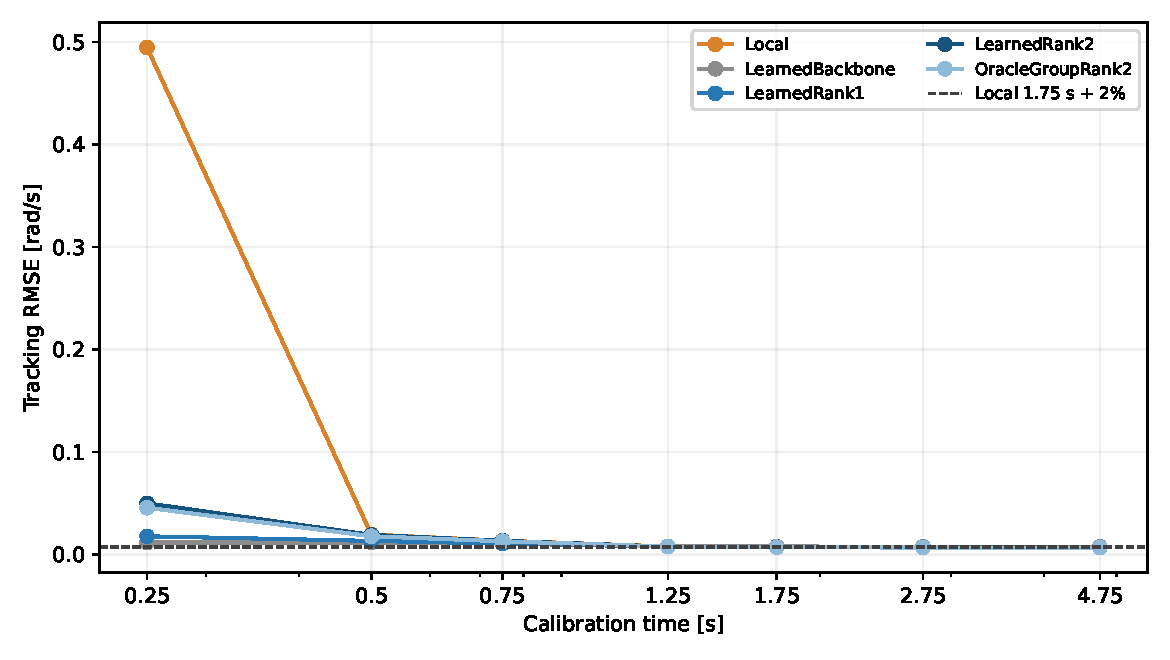
\includegraphics[width=0.84\linewidth]{../results/figures/experiment_9h_calibration_frontier.pdf}
\caption{Matched-prefix calibration frontier. Personalization protects the
information-limited client, while Local catches up once enough excitation is
available.}
\label{fig:experiment9h}
\end{figure}

\paragraph{Results: sharing solves cold start, not time to full quality.}
The primary gate fails. The 1.75~s Local reference is 0.007103 and its 2\%
tolerance is 0.007245, whereas Learned-rank-2 reaches only 0.007620 at 1.25~s.
Learned-rank-1, Learned-rank-2, and Local all first cross the target at the
measured 1.75~s budget. The experiment therefore does not show that
personalization reaches mature Local quality sooner.

At matched short budgets, however, sharing gives a large and consistent
advantage. At 0.50~s the shared backbone and rank-one model improve Local by
39.95\% and 31.79\%, respectively. At 0.75~s, rank one improves Local by
20.92\%; at 1.25~s, rank two improves it by 0.94\%. At 1.75~s both personalized
models are within 0.05\% of Local. Thus the benefit decreases continuously as
the local record becomes informative, exactly as expected for transferable
fleet knowledge.

The useful personalization rank is itself data dependent. With 0.25--0.50~s,
estimating two coordinates amplifies uncertainty and the zero-coordinate shared
backbone is best among deployable sharing methods. Rank one becomes best near
0.75~s, and rank two becomes competitive at 1.25~s. By 2.75~s, rank two and
Local both essentially reach Exact-individual tracking. This reveals a more
useful design than a fixed personalized head: uncertainty should activate local
degrees of freedom only when the available excitation supports them.

The very large 97.65\% relative improvement of the shared backbone over Local at
0.25~s should not be used as a headline percentage: the unconstrained three-
parameter Local fit is nearly unidentified and has tracking 0.4946. The 0.50--
0.75~s results are more representative evidence of cold-start protection. All
3900 parameter fits and all coefficient fits converge, and all 37,800 nonlinear
closed-loop evaluations remain feasible.

\paragraph{Decision.}
Experiment 9H supplies the missing reason to share information, but narrows the
claim. Personalized fleet learning does not outperform a sufficiently calibrated
Local model and does not reduce the observed time to the mature 1.75~s quality
threshold. It instead prevents severe identification and control degradation
during new-client cold start, then converges smoothly to Local performance.

The next method should therefore use uncertainty-gated personalization order:
start from a shared group backbone, activate the first client coordinate when
supported, and activate the second only after complementary excitation. This
directly combines the uncertainty-triggered acquisition of 9D with the
control-aware manifold of 9F. An end-to-end federated experiment should next
verify that distributed sufficient-statistic aggregation reproduces the shared
backbones under partial participation and should report the communication cost.
Privacy should be added only after that non-private protocol is frozen.

\paragraph{Reproducibility.}
The configuration is frozen in \path{code/config/experiment_9h.json}; the
implementation is \path{code/experiments/experiment_9h_calibration_frontier.py}.
Aggregate and seed-level curves, equal-budget improvements, log-time areas,
efficiency thresholds, assignments, and provenance are retained under
\path{results/tables}.
